\documentclass[11pt,letterpaper]{article}

\usepackage[margin=1in,letterpaper]{geometry}
\usepackage[T1]{fontenc}
\usepackage[utf8]{inputenc}
\usepackage{times}
\usepackage{amsmath}
\usepackage{amssymb}
\usepackage{array}
\usepackage{booktabs}
\usepackage{caption}
\usepackage{fancyhdr}
\usepackage{float}
\usepackage{hyperref}
\usepackage{listings}
\usepackage{setspace}
\usepackage{tabularx}
\usepackage{tikz}
\usepackage{xcolor}

\usetikzlibrary{arrows.meta, backgrounds, decorations.pathreplacing, fit, positioning}
\renewcommand{\ttdefault}{cmtt}

\singlespacing
\raggedright
\setlength{\parindent}{0pt}
\setlength{\parskip}{2pt}
\setlength{\headheight}{14pt}
\setlength{\textfloatsep}{8pt plus 1pt minus 2pt}
\setlength{\intextsep}{8pt plus 1pt minus 2pt}
\setlength{\abovecaptionskip}{4pt}
\setlength{\belowcaptionskip}{0pt}
\setlength{\abovedisplayskip}{6pt}
\setlength{\belowdisplayskip}{6pt}
\setlength{\emergencystretch}{2em}

\pagestyle{fancy}
\fancyhf{}
\fancyhead[C]{MASFE: An Onboard Multi-Algorithm Scheduling and Fusion Engine}
\fancyhead[R]{May 4, 2026}
\fancyfoot[R]{\thepage}
\renewcommand{\headrulewidth}{0.4pt}
\renewcommand{\footrulewidth}{0pt}

\makeatletter
\renewcommand\section{\@startsection{section}{1}{\z@}
  {0.55\baselineskip}
  {0.15\baselineskip}
  {\normalfont\large\bfseries}}
\renewcommand\subsection{\@startsection{subsection}{2}{\z@}
  {0.35\baselineskip}
  {0.1\baselineskip}
  {\normalfont\normalsize\bfseries}}
\makeatother

\definecolor{codeblue}{RGB}{0,90,160}
\definecolor{codegray}{RGB}{100,100,100}
\definecolor{codegreen}{RGB}{0,110,50}
\definecolor{codered}{RGB}{160,30,30}

\lstdefinestyle{masfe}{
  backgroundcolor=\color{gray!6},
  commentstyle=\color{codegreen},
  keywordstyle=\color{codeblue}\bfseries,
  stringstyle=\color{codered},
  basicstyle=\ttfamily\footnotesize,
  breakatwhitespace=false,
  breaklines=true,
  keepspaces=true,
  numbers=left,
  numbersep=8pt,
  numberstyle=\tiny\color{codegray},
  showspaces=false,
  showstringspaces=false,
  showtabs=false,
  tabsize=2,
  frame=single,
  rulecolor=\color{gray!40},
  captionpos=b
}
\lstset{style=masfe}
\renewcommand{\arraystretch}{1.15}
\newcommand{\masferepo}{https://github.com/emillambert/Emil_MASFE}

\begin{document}
\thispagestyle{fancy}

% Single-file source of truth for the Overleaf-ready paper.
\begin{center}
{\LARGE\bfseries MASFE: An Onboard Multi-Algorithm Scheduling and Fusion Engine}\\[2pt]
{\large For Regenerative Agriculture SmallSat Missions}\\[3pt]
Emil Wes Lambert, BSc Aerospace Engineering, TU Delft\\
Solo submission
\end{center}

\section{Introduction}

MASFE (Multi-Algorithm Scheduling and Fusion Engine) answers NASA's Space-to-Soil challenge by moving land-observation orchestration onboard instead of treating the spacecraft as a passive camera \cite{nasa-challenge-brief}. The target use case is regenerative agriculture, where disease and irrigation stress must be detected early enough for patch-level intervention instead of blanket chemical application. Current land products are typically too slow or too coarse for that workflow.

The proposed contribution is a two-stage, MDP-formulated scheduling policy executed as a deterministic, flight-verifiable rule set on a LEON4FT processor. A low-cost spectral screen runs every pass, and confirmation fuses thermal and moisture cues only when the belief state indicates likely stress. The payload is hosted on Loft Orbital's YAM platform with alerts to agricultural software via OpenET-linked ground services \cite{mytkowicz-webinar2,openet-api}; end-to-end architecture and the code submission URL are given in \S\ref{sec:solution}.

\begin{table}[H]
\centering
\caption{MASFE response to all five judging criteria.}
\label{tab:criteria-summary}
\begingroup
\small
\setlength{\tabcolsep}{5pt}
\renewcommand{\arraystretch}{1.1}
\begin{tabularx}{\linewidth}{p{2.2cm}p{3cm}X}
\toprule
\textbf{Criterion} & \textbf{Where} & \textbf{Key evidence} \\
\midrule
Creativity & \S2--3 & Beta-posterior scheduler, 3-channel CSC (EVI/LST/NDWI), EO-1 autonomy context. \\
Feasibility & \S2--3 & \S2; SWAP and compute in Table~\ref{tab:req-results}; MODIS replay in \S\ref{sec:impact}. \\
Impact & \S3 & Table~\ref{tab:req-results} and \S\ref{sec:impact} (downlink, energy, recall, FP). \\
Business & \S4 & Y1--Y5 rollout, Y3 profitability, FieldView/Deere/xarvio, international reach. \\
Presentation & Eq.~\eqref{eq:csc}, Fig.~\ref{fig:architecture}, \S\ref{sec:solution} & Architecture, CSC equation, reproducible simulation submission. \\
\bottomrule
\end{tabularx}
\endgroup
\end{table}

\section{Proposed Solution Detail}
\label{sec:solution}

MASFE uses a two-stage adaptive sensing loop. Stage 1 executes an EVI anomaly screen derived from MOD13A1 logic on every observed field patch and updates a per-patch stress posterior using EVI and NDWI cues from the same MSI acquisition. When the posterior indicates likely stress, Stage 2 runs a thermal retrieval derived from MOD11A1 and fuses EVI, LST, and MOD09A1-derived NDWI into a Crop Stress Composite (CSC), a normalized anomaly index conceptually related to temperature--vegetation dryness indices (e.g., TVDI) \cite{mod13a1,mod11a1,mod09a1,mod09-guide}. Only confirmed anomalous tiles are buffered for priority downlink. This makes sensing content-driven rather than timeline-driven and distinguishes MASFE from ASPEN/CASPER-style planners, which optimize scheduled activities rather than per-patch stress belief \cite{jpl-scheduling,eo1-autonomy}.

\begin{equation}
\text{CSC} = 0.40 \cdot \text{clip}\!\left(\frac{\Delta\text{EVI}}{5\sigma_e}, 0, 1\right)
           + 0.35 \cdot \text{clip}\!\left(\frac{\Delta\text{LST}}{4\sigma_l}, 0, 1\right)
           + 0.25 \cdot \text{clip}\!\left(\frac{\Delta\text{NDWI}}{4\sigma_n}, 0, 1\right)
\label{eq:csc}
\end{equation}

Here $\Delta\text{EVI} = \max(0, \text{EVI}_{base} - \text{EVI}_{obs})$, $\Delta\text{LST} = \max(0, \text{LST}_{obs} - \text{LST}_{base})$, and $\Delta\text{NDWI} = \max(0, \text{NDWI}_{base} - \text{NDWI}_{obs})$. The factors of $5$, $4$, and $4$ are simulation-calibrated saturation constants with an agronomic interpretation as the expected upper bounds of healthy seasonal EVI variability, thermal variability, and short-wave moisture variability for the tested crop regime; they map anomaly magnitude into $[0,1]$ before CSC composition. They are therefore tunable hyperparameters rather than fixed physical constants and would be re-calibrated on flight and field data. The implementation is intentionally deterministic even though the policy is MDP-formulated: that choice favors flight qualification and traceable verification on LEON4FT hardware over a learned black-box controller.

The scheduling logic is modeled as a finite-horizon MDP with per-patch Beta posteriors $\text{Beta}(\alpha_i,\beta_i)$ over stress probability. Stage~1 increments $\alpha_i$ when EVI or NDWI exceedance is observed and $\beta_i$ otherwise, with the evidence window capped to preserve responsiveness. Action selection compresses that patchwise belief into a mission state vector $s = (\mu_{\max}, \tau_{\max}, \text{SOC}, d, k)$, where $\mu_{\max}$ is the maximum posterior mean, $\tau_{\max}$ is the maximum $P(p > 0.5)$ tail probability, SOC is battery state of charge, $d \in \{0,1\}$ indicates downlink availability, and $k$ counts passes since last fusion. The action set remains \{SKIP, MOD13, FUSE, FUSE\_PRIORITY\}; NDWI is derived from the same MSI acquisition rather than requiring a separate action. The reward trades information gain against energy cost and missed-alert risk. The deployed solver is a hand-tuned deterministic policy that approximates the Bellman-optimal solution, chosen over learned policies because radiation-tolerant CPUs cannot justify neural inference at acceptable V\&V cost.

\begin{table}[H]
\centering
\caption{Mission requirements and demonstrated MASFE results.}
\label{tab:req-results}
\begin{tabularx}{\linewidth}{p{3.2cm}X}
\toprule
\textbf{Requirement} & \textbf{MASFE response} \\
\midrule
Alert latency $\leq$ 90 min & One-pass onboard screening, fusion, and alerting pipeline with X-band priority downlink. \\
Spatial resolution $\leq$ 30 m GSD & Tiered GSD pyramid: 30\,m screening on all passes, 10\,m confirmation on suspect patches, and 4.6\,m native evidence tiles for priority alerts. \\
False-positive rate $\leq$ 15\% & 1.6\% with benign confounders and roughly 30\% cloud-obscured passes per seed (\S\ref{sec:impact}). \\
SmallSat SWAP compliance & 9.6 W peak, 5.05 W duty-cycled payload average, 92.5\% peak LEON4FT ceiling, 39.2\% Stage-1 load, 49.2\% seasonal-average compute, and 86\% minimum state of charge in a local 40 Wh battery buffer. \\
Downlink efficiency & 99.3\% reduction versus raw downlink baseline while retaining 100\% disease-event recall (\S\ref{sec:impact}). \\
\bottomrule
\end{tabularx}
\end{table}

Average delivered resolution is therefore bandwidth-adaptive rather than fixed: screening remains coarse and cheap, while only high-priority evidence tiles preserve native sampling.

\begin{figure}[H]
\centering
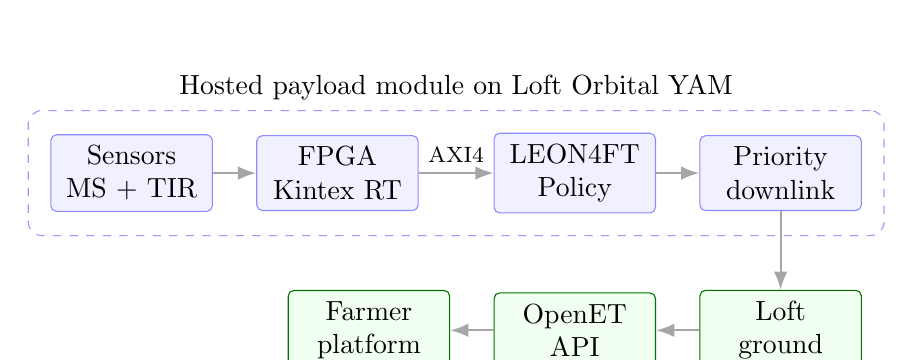
\begin{tikzpicture}[
  box/.style={
    draw, rounded corners=2pt, align=center,
    minimum height=0.95cm, minimum width=2.05cm,
    inner sep=4pt, font=\normalsize
  },
  sat/.style={box, fill=blue!6, draw=blue!45},
  grd/.style={box, fill=green!6, draw=green!45!black},
  arr/.style={-Latex, thick, draw=gray!70}
]

% Onboard (satellite) row
\node[sat]                           (sensor) {Sensors\\MS + TIR};
\node[sat, right=0.55cm of sensor]   (fpga)   {FPGA\\Kintex RT};
\node[sat, right=0.95cm of fpga]     (cpu)    {LEON4FT\\Policy};
\node[sat, right=0.55cm of cpu]      (tx)     {Priority\\downlink};

% Ground row
\node[grd, below=1.0cm of tx]        (ground) {Loft\\ground};
\node[grd, left=0.55cm of ground]    (openet) {OpenET\\API};
\node[grd, left=0.55cm of openet]    (farmer) {Farmer\\platform};

% Arrows
\draw[arr] (sensor) -- (fpga);
\draw[arr] (fpga)   -- node[above, font=\footnotesize] {AXI4} (cpu);
\draw[arr] (cpu)    -- (tx);
\draw[arr] (tx)     -- (ground);
\draw[arr] (ground) -- (openet);
\draw[arr] (openet) -- (farmer);

% Hosted payload bounding box
\begin{scope}[on background layer]
  \node[
    draw=blue!40, dashed, rounded corners=5pt,
    fit=(sensor)(fpga)(cpu)(tx), inner sep=8pt,
    label={[font=\normalsize]above:Hosted payload module on Loft Orbital YAM}
  ] {};
\end{scope}

\end{tikzpicture}
\caption{MASFE end-to-end architecture from onboard sensing to farmer alert delivery.}
\label{fig:architecture}
\end{figure}

The FPGA performs radiometric preprocessing and per-pixel CSC computation, then transfers frames to the LEON4FT over AXI4-Stream in under 1 ms. Onboard preprocessing includes radiometric calibration and cloud screening, while CSC itself is evaluated as a pass-to-pass relative anomaly detector rather than a fully atmosphere-corrected retrieval; full atmospheric correction is deferred to later validation because CSC is used for change detection rather than absolute retrieval. The selected Kintex UltraScale+ RT part comes from AMD's radiation-tolerant XQR family, specified to 100 krad total ionizing dose and QML-oriented qualification flows rather than commercial-grade testing \cite{amd-xqr}. MASFE is framed as a hosted payload module within a Loft Orbital YAM bus rather than as a full standalone 6U satellite; the SWAP budget therefore describes the payload module itself, not the host spacecraft. Spacecraft bus functions such as ADCS, OBC, and platform communications are provided by YAM, while MASFE carries a local 40 Wh battery and power-conditioning stage to preserve autonomy through eclipse periods and peak compute windows (40 Wh / 5.05 W $\approx$ 7.9 h, comfortably above the $\sim$35 min eclipse at 500 km SSO).

Operational degradation is explicit. Above 35\% battery state of charge, MASFE runs the full two-stage policy. Between 15\% and 35\%, it falls back to Stage 1 screening only. Below 15\%, it preserves energy for stored alert downlink. This satisfies the challenge requirement to degrade gracefully under onboard resource stress.

The quoted 92.5\% LEON4FT figure is a worst-case simultaneous-execution ceiling rather than a continuous load. Stage~1 alone occupies 39.2\% of LEON4FT capacity, while the upgraded action mix from the benchmark in \S\ref{sec:impact} yields a 49.2\% seasonal-average utilization because 81.3\% of synthetic passes remain at 30\,m screening and only 18.7\% escalate to full fusion. That leaves meaningful headroom for RTOS, watchdog, and fault-handling overhead while making hardware-in-the-loop timing validation the right next step.

Each priority alert packet contains a geo-tagged field-patch polygon with centroid coordinates, CSC severity score, contributing EVI/LST/NDWI anomaly components, timestamp and pass ID, and a confidence flag derived from consecutive confirming passes. Priority evidence tiles are compressed onboard using CCSDS 122.0 wavelet coding with a planning assumption of roughly 2.5:1, reducing a nominal 8.4\,MB/km$^2$ native alert stream to about 3.36\,MB/km$^2$ delivered before packetization \cite{esa-cwicom}. Per-patch geolocation is derived from bus ephemeris and attitude solutions and is budgeted to remain comfortably inside the 30\,m effective-GSD requirement. These packets are delivered through Loft Orbital's ground network to farm software as geo-tagged overlays via the OpenET-linked API, enabling push notifications within 15 minutes of contact.

Full simulation source code (\texttt{masfe\_simulation.py}) is submitted as Code Component 3 at \href{\masferepo}{github.com/emillambert/Emil\_MASFE}.

\section{Potential Impact}
\label{sec:impact}

MASFE does not introduce a new crop model; it orchestrates standard land-product evidence as laid out in \S\ref{sec:solution}. That prioritization matters for time-sensitive decisions. Dr.\ Katie Gold's disease-detection work emphasizes that spectral stress often appears before visible symptoms and before whole-field treatment would be agronomically or economically rational \cite{gold-webinar1}.

In a 100-seed Monte Carlo benchmark, MASFE was tested over 120 passes, 500 field patches, 21 disease events, and 9 benign confounders per seed, with roughly 36.7 cloud-obscured passes per seed. Relative to raw downlink, it reduced transmitted data by 99.3\% and active payload energy by 38.6\%. Relative to a fixed onboard pipeline, the Bayesian belief gate adds volumetric and operational value together: versus always-on fusion, MASFE cuts downlinked data by 80.7\% and payload energy by 24.6\% while keeping the pass mix skewed toward Stage~1 screening (\S\ref{sec:solution}). Mission usefulness remained strong: disease-event recall stayed at 100.0\%, alert precision reached 98.4\%, and the false-positive rate remained at 1.6\%.

Across that benchmark, 95\% confidence intervals were 99.32--99.33\% for downlink reduction versus raw, 38.52--38.70\% for energy saving versus raw, 100.0--100.0\% for disease-event recall, and 1.34--1.78\% for false-positive rate. The operating point is tunable: sweeping $csc\_alert\_thr$ from 0.40 to 0.70 preserved 100.0\% recall until the most conservative endpoint while moving false-positive rate from 2.23\% to 1.26\%, and a $\pm30\%$ CSC-parameter sweep kept recall at 100.0\% with false-positive rate in the 1.0--2.3\% band; detailed curves and cases are included in the code submission.

A matched-recall ablation that removes the Bayesian belief memory and reacts only to current-pass anomalies increases false-positive rate from 1.6\% to 1.7\% while driving seasonal compute from 49.2\% to 76.2\%. In other words, the posterior is load-bearing primarily as a scheduler: it preserves recall while sharply reducing unnecessary Stage~2 execution.

The code component now also replays official MOD13A1 and MOD11A1 subsets over Westlands/Firebaugh, California, from June through October 2024. That run aligns MOD13A1 composite dates to a 1 km grid, collapses MOD11A1 to median clear-sky daytime LST over the same 16-day window, and applies the unchanged MASFE policy as a real-scene scheduler validation rather than a labeled disease benchmark. The replay path now also accepts MOD09A1-derived NDWI where available, but the tracked Westlands anchor bundle predates that extension and therefore falls back cleanly to EVI/LST fusion on the cached artifacts. Across 7 valid composite windows after a 3-window warmup, MASFE issued one confirmed FUSE\_PRIORITY alert on July 27, 2024 and six additional FUSE-only windows at 99.5\% mean valid coverage.

The farm-scale value proposition is concrete. For a 500 ha regenerative tomato operation, blanket preventative fungicide at roughly \$85/ha per application implies about \$39{,}000/season of avoidable chemical spend if MASFE confines treatment to the roughly 8\% of the field flagged during an event. That matters because late blight remains a destructive tomato disease that can destroy entire fields and collapse plants within 7--10 days under cool, wet conditions \cite{wisconsin-lateblight}. At the Y3 U.S.-scale rollout of 2.5 Mha, the same \$78/ha treatment-deferral arithmetic implies a gross pre-adoption potential of roughly \$195\,M/season in avoided blanket fungicide spend before yield protection is counted.

The main limitations are honest rather than hidden. The current headline metrics are still anchored in synthetic proxy data, while the real-scene replay is designed to validate scheduler behavior on official products rather than claim field-labeled disease accuracy. Tropical crop calendars would still require policy recalibration, but that is a validation gap rather than an architectural gap.

\section{Team Experience and Market Evaluation}

MASFE is a solo submission, so credibility comes from systems execution rather than headcount. Emil Wes Lambert is completing a BSc in Aerospace Engineering at TU Delft, with coursework across spacecraft systems engineering, AOCS, mission analysis, and embedded flight software. At AeroDelft he has led partnerships and business operations, including procurement, sponsor relations, and participation in the €73 M HAPSS hydrogen-propulsion consortium alongside Airbus, KLM, NLR, and other industrial partners. That combination maps onto MASFE's SWAP realism, AIST-track funding strategy, and hosted-payload commercial positioning.

The commercial case is broader than a single California valley: the San Joaquin Valley anchors the replay validation in \S\ref{sec:impact}, not the total addressable market. The same architecture scales from SJV into the wider U.S. irrigated base, then into EU and Brazilian irrigation markets, and finally into a global irrigated-farmland platform without changing the onboard payload logic \cite{usda-2022,eurostat-farms,ana-atlas,fao-aquastat}. The paper-facing economics therefore use a low/design-to-cost hosted-payload case, a \$4/ha/year alerting product, a modeled 90\% annual retention rate, and a Year~2 soil-carbon MRV add-on aligned to Verra VM0042-style workflows \cite{climate-pricing,verra-vm0042}.

\begin{table}[H]
\centering
\caption{MASFE rollout from SJV pilot to global platform (low/design-to-cost case); Westlands replay in \S\ref{sec:impact}.}
\label{tab:unit-econ}
\small
\begin{tabular}{llp{2.15cm}lrr}
\toprule
Year & Milestone & Geography & Coverage & Revenue & Op. margin \\
\midrule
Y1 & SJV pilot & California SJV & 3.5\% SJV & \$0.20\,M & \shortstack[r]{grant-funded} \\
Y2 & California scale & California & 28.3\% SJV & \$1.70\,M & 17.1\% \\
Y3 & U.S. national & U.S. irrigated & 11.0\% US & \$10.62\,M & 60.4\% \\
Y4 & EU + Brazil entry & EU + Brazil & 35.1\% EU+Brazil & \$27.62\,M & 68.1\% \\
Y5 & Global platform & Global & 6.0\% global & \$76.50\,M & 70.7\% \\
\bottomrule
\end{tabular}
\end{table}

In this rollout, Y1 is a paid pilot (replay context in \S\ref{sec:impact}), Y2 scales through Climate FieldView plus direct enterprise sales, Y3 reaches U.S.-scale profitability through Climate FieldView and John Deere Operations Center, Y4 enters EU and Brazilian markets through xarvio and John Deere Brazil, and Y5 becomes a global multi-platform product that can also flow through CropX. Y1 is intentionally modeled as an AIST- or NASA SBIR/STTR-style co-funded bridge-to-MVP year rather than a self-financing steady state \cite{nasa-aist,nasa-sbir}. Base and high fixed-cost sensitivities still break even at Y3 and 2.5\,Mha. At constellation scale, three YAM-hosted payloads would reduce revisit from roughly 90 minutes to roughly 30 minutes, and a Stage~1 anomaly on one pass could cue a Stage~2 priority acquisition on the next satellite.

That generalization story matters for the judges' business-model criterion. Agriculture is the entry market, but the same scheduling core can be retuned for wildfire fuel-moisture monitoring, a forest-wildfire detection market projected to reach about \$950\,M by 2032 \cite{wildfire-market}; flood-front tracking would swap CSC for water-extent products, and urban heat-island response would replace farm polygons with city blocks while reusing the same anomaly-driven scheduler.

\section{Expected Next Steps}

MASFE is currently a TRL 3 concept: the scheduling logic, fusion equation, SWAP closure, and real-scene replay are demonstrated in software, but the payload has not yet been exercised on target hardware. The next milestone is a TRL 4 hardware-in-the-loop demonstration on a LEON4FT-class evaluation platform under the NASA AIST (Advanced Information Systems Technology) instrument demonstration pathway using the replayed EarthData scene set. TRL-4 hardware work should also add FPGA-side Fmask-style Stage~0 cloud screening, replacing the current software approximation used in the replay path. After that, the cleanest TRL 5 path is a hosted-payload pilot through Loft Orbital, with external validation focused on the Y1 paid-pilot assumptions, agronomy review, and distribution-partner plausibility.

\section{Conclusion}

\label{chapter:conclusion}

MASFE demonstrates that adaptive sensing and onboard processing can transform SmallSat missions from passive collectors into responsive decision systems. The two-stage Markov Decision Process (MDP) scheduling policy reuses standard land-product evidence and escalates fusion only when the belief state warrants it (\S\ref{sec:solution}), achieving the headline downlink, energy, recall, and false-positive performance summarized in Table~\ref{tab:req-results} and \S\ref{sec:impact}, within hosted-payload SWAP constraints. For regenerative agriculture, that means shifting from blanket preventative treatment to targeted, evidence-based intervention at field-patch scale. More broadly, MASFE contributes a reusable onboard orchestration primitive that can extend beyond agriculture into other anomaly-driven Earth-observation missions.

\clearpage
\footnotesize
\begin{thebibliography}{99}
\setlength{\itemsep}{0.1em}
\setlength{\parskip}{0pt}

\bibitem{nasa-challenge-brief}
NASA Earth Science Technology Office,
\emph{Space-to-Soil Challenge: Challenge Brief and Guidelines},
2026.
\url{https://nasa-space-to-soil.org}.

\bibitem{mod13a1}
NASA EOSDIS Land Processes DAAC,
\emph{MOD13A1 MODIS/Terra Vegetation Indices 16-Day L3 Global 500 m SIN Grid V061},
2021.
DOI: \url{https://doi.org/10.5067/MODIS/MOD13A1.061}.

\bibitem{mod11a1}
NASA EOSDIS Land Processes DAAC,
\emph{MOD11A1 MODIS/Terra Land Surface Temperature/Emissivity Daily L3 Global 1 km SIN Grid V061},
2021.
DOI: \url{https://doi.org/10.5067/MODIS/MOD11A1.061}.

\bibitem{mod09a1}
E. Vermote,
\emph{MODIS/Terra Surface Reflectance 8-Day L3 Global 500m SIN Grid V061},
NASA Land Processes Distributed Active Archive Center, 2021.
DOI: \url{https://doi.org/10.5067/MODIS/MOD09A1.061}.

\bibitem{mod09-guide}
MODIS Land Surface Reflectance Science Computing Facility,
\emph{MODIS Surface Reflectance User's Guide, Collection 6},
2020.
\url{https://www.earthdata.nasa.gov/s3fs-public/2025-04/MOD09_User_Guide_V61.pdf}.

\bibitem{gold-webinar1}
K. Gold,
\emph{Spectral Early Detection of Crop Pathogens for Regenerative Agriculture Applications},
NASA Space-to-Soil Challenge Informational Webinar 1,
Cornell University Plant Disease Diagnostics Laboratory, February 12, 2026.

\bibitem{mytkowicz-webinar2}
J. Mytkowicz,
\emph{AI-Enabled Satellites and On-Orbit Decision-Making: Lessons from Loft Orbital},
NASA Space-to-Soil Challenge Informational Webinar 2,
Loft Orbital, March 25, 2026.

\bibitem{openet-api}
OpenET Consortium,
\emph{FARMS API Documentation},
2025.
\url{https://openet.gitbook.io/docs/additional-resources/farms}.

\bibitem{jpl-scheduling}
JPL Artificial Intelligence Group,
\emph{Scheduling and Planning Technology},
2024.
\url{https://ai.jpl.nasa.gov/public/projects/}.

\bibitem{eo1-autonomy}
R. Sherwood, S. Chien, D. Tran, R. Castano, and others,
\emph{Intelligent Systems in Space: The EO-1 Autonomous Sciencecraft},
NASA Technical Reports Server, 2005.
\url{https://ntrs.nasa.gov/citations/20060044325}.

\bibitem{usda-2022}
USDA National Agricultural Statistics Service,
\emph{2022 Census of Agriculture: United States Summary and State Data},
2024.
\url{https://www.nass.usda.gov/Publications/AgCensus/2022/Full_Report/Volume_1\%2C_Chapter_1_US/usv1.pdf}.

\bibitem{eurostat-farms}
Eurostat,
\emph{Farms and Farmland in the European Union},
Statistics Explained, 2025.
\url{https://ec.europa.eu/eurostat/statistics-explained/index.php?title=Farms_and_farmland_in_the_European_Union}.

\bibitem{ana-atlas}
Agencia Nacional de Aguas e Saneamento Basico,
\emph{Atlas Irrigacao},
2021.
\url{https://www.ana.gov.br/atlasirrigacao/}.

\bibitem{fao-aquastat}
FAO AQUASTAT,
\emph{Irrigated Areas and Water Use: Conclusions},
2025.
\url{https://www.fao.org/aquastat/en/data-analysis/irrig-water-use/conclusions/}.

\bibitem{climate-pricing}
Climate FieldView,
\emph{FieldView Pricing},
2026.
\url{https://climate.com/pricing}.

\bibitem{amd-xqr}
AMD,
\emph{Kintex UltraScale XQR Radiation-Tolerant FPGA Family},
2026.
\url{https://www.amd.com/en/products/adaptive-socs-and-fpgas/fpga/kintex-ultrascale-xqr.html}.

\bibitem{esa-cwicom}
European Space Agency,
\emph{CCSDS Image Data Compression ASIC},
2026.
\url{https://www.esa.int/Enabling_Support/Space_Engineering_Technology/Onboard_Data_Processing/CCSDS_Image_Data_Compression_ASIC}.

\bibitem{nasa-aist}
NASA Earth Science Technology Office,
\emph{Advanced Information Systems Technology and ESTO Funding Process},
2026.
\url{https://esto.nasa.gov/funding-process/}.

\bibitem{nasa-sbir}
NASA,
\emph{Small Business Innovation Research / Small Business Technology Transfer},
2026.
\url{https://www.nasa.gov/sbir_sttr/}.

\bibitem{wisconsin-lateblight}
University of Wisconsin Horticulture,
\emph{Late Blight},
2024.
\url{https://hort.extension.wisc.edu/articles/late-blight/}.

\bibitem{wildfire-market}
Future Market Report,
\emph{Forest Wildfire Detection System Market Size, Share, Growth and Forecast to 2032},
2026.
\url{https://www.futuremarketreport.com/industry-report/forest-wildfire-detection-system-market}.

\bibitem{verra-vm0042}
Verra,
\emph{VM0042 Methodology for Improved Agricultural Land Management},
2025.
\url{https://verra.org/methodologies/vm0042-methodology-for-improved-agricultural-land-management-v2-0/}.

\end{thebibliography}

\end{document}
